\documentclass[runningheads]{llncs}
\usepackage[T1]{fontenc}
\usepackage{lmodern}
\usepackage{microtype}
\usepackage[hidelinks]{hyperref}
\usepackage{pgfplots}
\usepackage{ragged2e} 
\usepackage{comment}


\pgfplotsset{compat=1.17}

\renewcommand{\UrlFont}{\small\ttfamily} 

\sloppy

\titlerunning{Deep Learning Approaches for Alzheimer’s Classification}
\title{Deep Learning Approaches for Alzheimer’s Disease Classification Using MRI Images}
\author{Rareș-Andrei Filip\inst{1} \and Dragoș Ilieș\inst{1}}
\institute{
Faculty of Economics and Business Administration (FSEGA), \\
Babeș-Bolyai University (UBB), Cluj-Napoca, Romania
}

\begin{document}
\maketitle
\pagestyle{plain}

\begin{abstract}
    Alzheimer's Disease (AD) is a progressive neurodegenerative disorder that affects memory and cognitive functions. Early detection is essential for slowing disease progression and improving patient outcomes. This study investigates the performance of various machine learning (ML) and deep learning (DL) models in classifying Alzheimer's stages using MRI images. The dataset comprises four classes: Non-Demented, Very Mild Demented, Mild Demented, and Moderate Demented.

    Traditional ML methods, including Support Vector Machines (SVM) and Random Forest, were compared with advanced DL models such as Convolutional Neural Networks (CNN) and ResNet. Results indicate that SVM achieved the highest accuracy among all methods, demonstrating the efficiency of classical ML techniques for this dataset. CNN and ResNet, while slightly less accurate, showed potential for handling larger and more complex datasets.

    This study underscores the strengths of ML and DL approaches and suggests that their combination could enhance diagnostic performance for Alzheimer's Disease.
    \keywords{Alzheimer's Disease, Deep Learning, Machine Learning, Convolutional Neural Networks, Support Vector Machines, ResNet.}
\end{abstract}

\section{Introduction}

Alzheimer's Disease (AD) is a neurodegenerative disorder that progressively deteriorates memory, cognitive abilities, and daily functioning. It is the leading cause of dementia, representing 60–80\% of cases globally~\cite{helaly2021}. Recent data shows that over 50 million people worldwide are living with AD, a number projected to reach 152 million by 2050. Identifying the disease in its early stages is essential for slowing its progression and improving patient care.

Magnetic Resonance Imaging (MRI) plays a crucial role in detecting brain changes linked to AD. Structural alterations in regions like the hippocampus and gray matter are key indicators of early-stage disease. However, traditional methods of MRI analysis rely on manual evaluation and handcrafted feature extraction, which are labor-intensive and prone to inconsistencies.

Advances in Artificial Intelligence (AI), particularly Deep Learning (DL), have transformed medical imaging. Models like Convolutional Neural Networks (CNNs) excel in feature extraction and classification tasks, often outperforming manual approaches. Additionally, techniques such as transfer learning enhance performance, especially when working with limited datasets.

Despite these advancements, several questions remain:
\begin{itemize}
    \item Can machine learning and deep learning models reliably classify Alzheimer's stages?
    \item How do traditional machine learning methods, like Support Vector Machines (SVM) and Random Forest, compare to deep learning models such as CNN and ResNet in terms of accuracy and computational efficiency?
    \item What practical value can these models provide to clinicians for supporting early diagnosis in real-world environments?
\end{itemize}

This study aims to address these questions by comparing the performance of machine learning and deep learning models for Alzheimer's classification. The focus is on evaluating their accuracy, strengths, and limitations, while identifying opportunities for combining these approaches to improve diagnostic capabilities.

\section{Related Work}

Many studies have investigated the use of machine learning (ML) and deep learning (DL) for classifying Alzheimer's Disease (AD) stages using MRI data.

Helaly et al.~\cite{helaly2021} used transfer learning with pre-trained CNN models like VGG19 to classify MRI scans into different AD stages. They showed that transfer learning reduces overfitting when data is limited. However, their work did not include attention mechanisms, which can enhance feature localization.

Nasir et al.~\cite{nasir2021} combined multiple CNN architectures into an ensemble model, achieving 90\% accuracy using majority voting. While effective, ensemble models often require significant computational resources, making them less practical for clinical use.

Pandiyaraju et al.~\cite{pandiyaraju2022} developed a dual-attention-aware CNN to focus on critical brain regions like the hippocampus. Their model achieved state-of-the-art accuracy of 99.1\%, highlighting the potential of attention mechanisms for better feature extraction.

Jo et al.~\cite{jo2021} combined MRI and PET data in a multimodal approach, using stacked autoencoders and CNNs to achieve accuracies over 98\%. This shows the advantage of integrating complementary imaging modalities for improved diagnosis.

Hybrid methods that combine ML and DL techniques have also been explored. Khvostikov et al.~\cite{khvostikov2022} used structural and diffusion imaging data with feature extraction techniques to improve accuracy. However, their reliance on manual feature engineering makes the approach time-consuming and error-prone.

In summary, existing methods demonstrate high accuracy but have limitations such as computational cost, dependence on large annotated datasets, and limited applicability in clinical settings. This study builds on previous work by comparing transfer learning, attention mechanisms, and hybrid frameworks to create a robust and efficient model for AD classification.

\section{Dataset Description}

The Alzheimer's MRI Disease Classification dataset~\cite{dataset_source} contains Magnetic Resonance Imaging (MRI) brain scans categorized into four classes: Non-Demented, Very Mild Demented, Mild Demented, and Moderate Demented. This dataset is suitable for our research as it includes labeled images that support both binary classification (Alzheimer's vs. Non-Alzheimer's) and multi-class classification tasks. By including different stages of Alzheimer's Disease (AD), the dataset enables a comprehensive evaluation of machine learning (ML) and deep learning (DL) methods.

The dataset provides grayscale 2D MRI images that highlight structural changes in the brain, such as hippocampal atrophy and gray matter loss, which are key indicators of AD progression. These labeled images are essential for supervised learning models and reflect real-world scenarios with class imbalance, making the dataset highly applicable for medical research.

Figure~\ref{fig:sample_images} shows sample images from the dataset, illustrating differences between the four classes.

\begin{figure}[htbp]
    \centering
    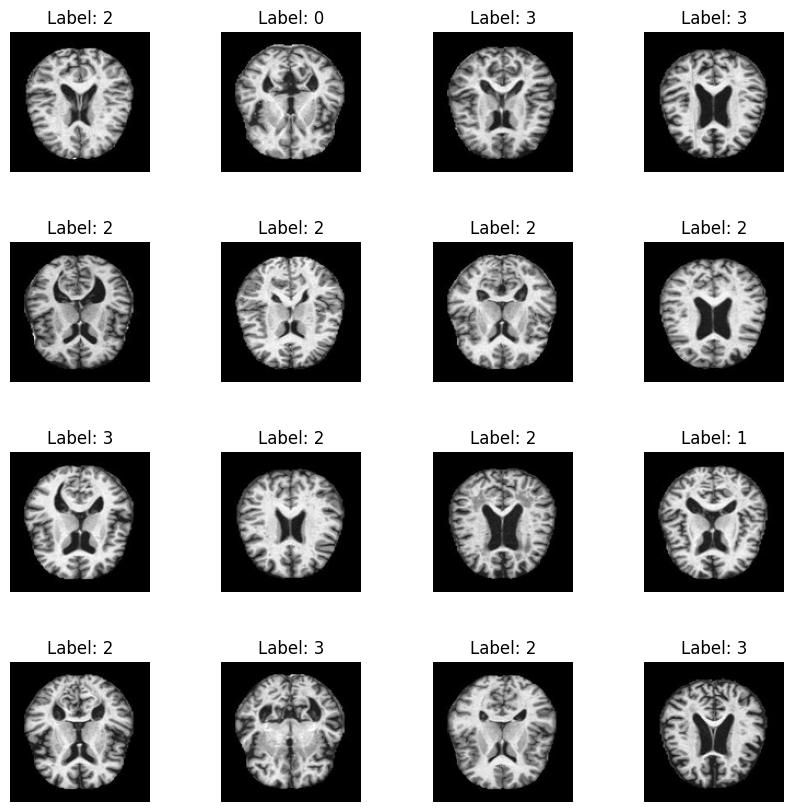
\includegraphics[width=0.8\textwidth]{C:/Users/Dragos/Documents/Deep learning/Alzheimer_Project/sample_image}
    \caption{Sample MRI images from the dataset.}
    \label{fig:sample_images}
\end{figure}

\subsection{Data Preprocessing}
The dataset was preprocessed to prepare the images for analysis. The main steps included:
\begin{enumerate}
    \item \textbf{Resizing:} All images were resized to $128 \times 128$ pixels to standardize input dimensions and reduce computational cost.
    \item \textbf{Normalization:} Pixel values were scaled to the range [0, 1] to improve model convergence during training.
    \item \textbf{Augmentation:} Techniques such as horizontal flipping, rotation, and scaling were applied to underrepresented classes (e.g., Moderate Demented) to address class imbalance.
\end{enumerate}

\subsection{Class Distribution}
The dataset contains an uneven number of images across the four classes. Figure~\ref{fig:class_distribution} shows the distribution, highlighting that the `Non-Demented` class has the most samples, while the `Moderate Demented` class has the least. This imbalance can bias models toward the majority class, so data augmentation was applied to mitigate its effects.

\begin{figure}[htbp]
    \centering
    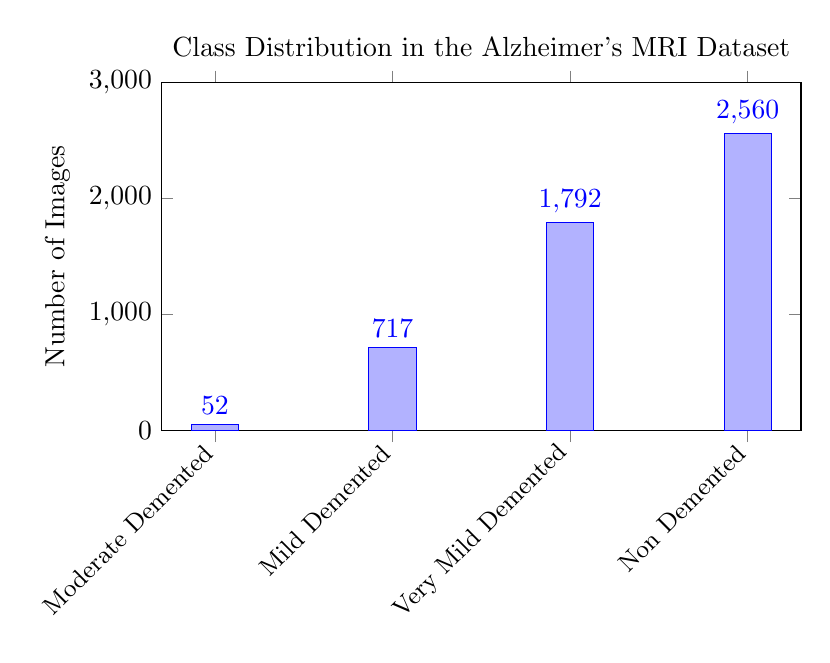
\begin{tikzpicture}
        \begin{axis}[
                ybar, % Vertical bars
                ymin=0, ymax=3000, % Y-axis range
                width=0.8\textwidth, % Width of the chart
                height=6cm, % Height of the chart
                xlabel={}, % X-axis title
                ylabel={Number of Images}, % Y-axis title
                symbolic x coords={Moderate Demented, Mild Demented, Very Mild Demented, Non Demented},
                xtick=data, % X-axis labels
                xticklabel style={font=\small, rotate=45, anchor=east}, % Rotate X-axis labels
                nodes near coords, % Show data labels
                nodes near coords align={vertical}, % Align data labels
                bar width=0.6cm, % Bar width
                title={Class Distribution in the Alzheimer's MRI Dataset}
            ]
            \addplot coordinates {(Moderate Demented,52) (Mild Demented,717) (Very Mild Demented,1792) (Non Demented,2560)};
        \end{axis}
    \end{tikzpicture}
    \caption{Distribution of Classes in the Alzheimer's MRI Dataset.}
    \label{fig:class_distribution}
\end{figure}

\section{Methodology}

This section describes the approaches used to classify data, including deep learning models (DNN, CNN, and ResNet) and traditional machine learning models (SVM and Random Forest). The key settings, validation strategies, and parameter selection methods for each model are detailed below.

\subsection{Deep Neural Network (DNN)}
The DNN was implemented as a fully connected feed-forward network with the following settings:
\begin{itemize}
    \item \textbf{Input Dimensions:} $128 \times 128 \times 3$ RGB images resized and flattened into 1D vectors.
    \item \textbf{Hidden Layers:}
          \begin{itemize}
              \item Layer 1: 512 neurons with ReLU activation.
              \item Layer 2: 256 neurons with ReLU activation.
              \item Layer 3: 128 neurons with ReLU activation.
          \end{itemize}
    \item \textbf{Dropout:} 50\% dropout was applied after the first two dense layers to prevent overfitting.
    \item \textbf{Output Layer:} A softmax layer for classification into four classes.
    \item \textbf{Optimizer:} Adam optimizer with a learning rate of $0.001$.
    \item \textbf{Loss Function:} Sparse Categorical Cross-Entropy.
    \item \textbf{Batch Size:} 32.
    \item \textbf{Epochs:} 10.
\end{itemize}
While the DNN model was computationally efficient due to its simplicity, its performance was significantly lower compared to the other methods.

\subsection{Baseline Convolutional Neural Network (CNN)}
The baseline CNN consisted of convolutional layers, max-pooling layers, and fully connected layers. It was trained using the following settings:
\begin{itemize}
    \item \textbf{Input Dimensions:} $128 \times 128 \times 3$ RGB images.
    \item \textbf{Activation Function:} ReLU.
    \item \textbf{Optimizer:} Adam with a learning rate of $0.0001$.
    \item \textbf{Batch Size:} 16.
    \item \textbf{Loss Function:} Sparse Categorical Cross-Entropy.
    \item \textbf{Epochs:} 20.
\end{itemize}
Overfitting was observed after 10 epochs, motivating the use of more advanced models.

\subsection{ResNet with Data Augmentation}
ResNet-50 was employed to improve performance. The model was initialized with ImageNet weights, and the following techniques were applied:
\begin{itemize}
    \item \textbf{Data Augmentation:} Rotation, flipping, and scaling.
    \item \textbf{Fine-Tuning:} The top layers were unfrozen after initial training.
    \item \textbf{Batch Size:} 8 (limited by available memory).
    \item \textbf{Epochs:} 20.
\end{itemize}
Due to memory limitations, further fine-tuning and testing on augmented data were not feasible.

\subsection{Support Vector Machines (SVM)}
An SVM classifier was trained using flattened feature vectors. The optimal regularization parameter \(C\) was selected via grid search with cross-validation. The best value was \(C=1\).

\subsection{Random Forest}
The Random Forest model was trained with the following settings:
\begin{itemize}
    \item \textbf{Number of Trees:} 100.
    \item \textbf{Max Depth:} Selected via grid search.
    \item \textbf{Criterion:} Gini Impurity.
\end{itemize}
This model offered interpretability but required feature extraction.

\subsection{Validation Strategy}
A 15\% split of the dataset was used for validation during model training. Test data were kept separate to evaluate model performance. Cross-validation was used for hyperparameter tuning in SVM and Random Forest.

\section{Results and Discussion}

This section evaluates the performance of the deep learning (DNN, CNN, ResNet) and machine learning models (SVM, Random Forest) for Alzheimer’s Disease classification. The results are analyzed with respect to accuracy, loss, and confusion matrices, while also addressing the challenges and potential future improvements.

\subsection{Performance Analysis}

Table~\ref{tab:performance_metrics} summarizes the performance metrics for all models. Among the methods tested, SVM achieved the highest test accuracy (98.2\%), followed by CNN (93.9\%) and Random Forest (91.6\%). ResNet and DNN underperformed due to computational limitations and inadequate feature learning.

\begin{table}[htbp]
    \centering
    \caption{Performance Metrics for All Models.}
    \label{tab:performance_metrics}
    \begin{tabular}{|c|c|c|c|}
        \hline
        \textbf{Model} & \textbf{Training Accuracy (\%)} & \textbf{Test Accuracy (\%)} & \textbf{Loss} \\
        \hline
        DNN            & 49.5                            & 49.5                        & 1.038         \\
        CNN            & 98.4                            & 93.9                        & 1.028         \\
        ResNet         & 62.5                            & 57.8                        & 0.886         \\
        SVM            & -                               & 98.2                        & -             \\
        Random Forest  & -                               & 91.6                        & -             \\
        \hline
    \end{tabular}
\end{table}

The DNN model achieved the weakest performance, with a test accuracy of 49.5\%. This was expected since the input data was prepared for CNN models, and DNN lacks the convolutional layers needed to capture spatial features in the images.

The CNN model demonstrated strong performance, leveraging convolutional layers to learn spatial patterns effectively. The test accuracy of 93.9\% validates its ability to classify Alzheimer’s stages. However, reducing training epochs from 20 to 10 led to slightly lower results, suggesting that overfitting was not a significant concern for this dataset.

ResNet, despite its powerful transfer learning capabilities, achieved a test accuracy of only 57.8\%. This performance was limited by computational constraints, which restricted batch sizes and prevented effective fine-tuning and data augmentation.

Traditional machine learning models also performed well. SVM outperformed all other models, achieving near-perfect classification (98.2\%), as shown in its confusion matrix (Figure~\ref{fig:svm_confusion}). Random Forest, while slightly less accurate (91.6\%), provided interpretability, demonstrating its utility for feature importance analysis.

\subsection{Confusion Matrix Interpretation}

Figures~\ref{fig:cnn_confusion} and~\ref{fig:svm_confusion} present the confusion matrices for CNN and SVM, respectively. These matrices illustrate the classification performance across the four stages of Alzheimer’s Disease.

\begin{figure}[htbp]
    \centering
    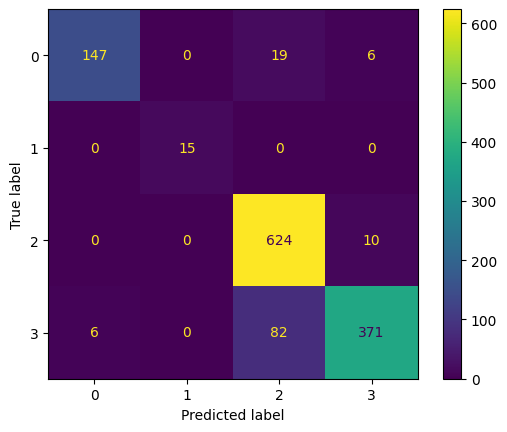
\includegraphics[width=0.7\textwidth]{cnn_confusion_matrix.png}
    \caption{Confusion Matrix for CNN.}
    \label{fig:cnn_confusion}
\end{figure}

\begin{figure}[htbp]
    \centering
    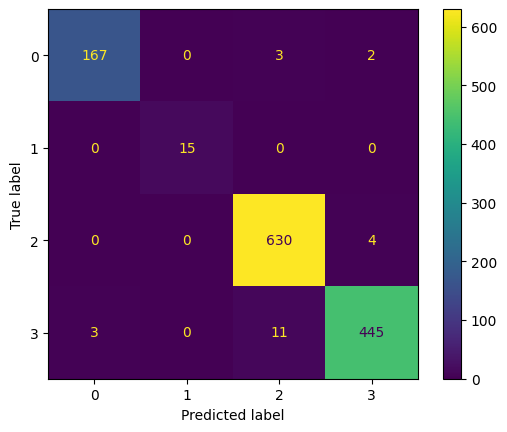
\includegraphics[width=0.7\textwidth]{svm_confusion_matrix.png}
    \caption{Confusion Matrix for SVM.}
    \label{fig:svm_confusion}
\end{figure}

The CNN confusion matrix (Figure~\ref{fig:cnn_confusion}) reveals that it correctly classified a large proportion of samples in all classes. For instance, in Class 2 (Mild Cognitive Impairment), the model classified 624 samples correctly out of the total 634. However, the CNN struggled more significantly with Class 3 (Severe Cognitive Impairment), misclassifying 82 samples into Class 2 and 6 samples into Class 0. This indicates that the CNN model, while effective at capturing spatial patterns, faced difficulties in distinguishing adjacent classes with overlapping characteristics.

In comparison, the confusion matrix for the SVM model  (Figure~\ref{fig:svm_confusion}) shows excellent performance across all classes. For Class 2, the SVM correctly classified 630 out of 634 samples, with only 4 samples misclassified. For Class 3, the model correctly identified 445 samples, with minor confusion leading to 11 samples being classified as Class 2. The SVM's overall performance demonstrates its robustness in effectively distinguishing between classes, even when the input features are flattened and spatial information is lost. This highlights the SVM's capacity to handle the task efficiently, leveraging its simplicity and well-defined hyperplane separation.

\subsection{Challenges and Limitations}

The main limitations encountered in this study include:

\begin{itemize}
    \item \textbf{Memory Constraints:} The limited RAM in the computational environment restricted the batch size and prevented effective fine-tuning and data augmentation for ResNet.
    \item \textbf{Dataset Size:} The relatively small dataset impacted the generalization capabilities of deep learning models, particularly ResNet.
    \item \textbf{Model Specificity:} Models like DNN were not well-suited for the spatial nature of the input data, resulting in poor performance.
\end{itemize}

\subsection{Future Work}

To address these limitations, future work could focus on:
\begin{itemize}
    \item \textbf{Larger Datasets:} Incorporating larger and more diverse datasets to enhance model generalization and robustness.
    \item \textbf{Ensemble Methods:} Exploring hybrid approaches combining CNN, SVM, and Random Forest for improved accuracy and interpretability.
    \item \textbf{Optimized Architectures:} Using lightweight architectures or distributed training methods to overcome memory constraints.
    \item \textbf{Clinical Integration:} Designing real-time, scalable models for clinical applications to support early diagnosis and treatment.
\end{itemize}

\subsection{Answering Research Questions}

This study addressed the following research questions:
\begin{itemize}
    \item \textbf{Can machine learning and deep learning models reliably classify Alzheimer’s stages?} Yes, both approaches demonstrated the capability to classify Alzheimer’s stages, with SVM achieving the highest accuracy and CNN showing strong potential for spatial feature learning.
    \item \textbf{How do traditional machine learning methods compare to deep learning models?} Traditional methods, particularly SVM, outperformed deep learning models in terms of accuracy. However, CNN excelled in leveraging spatial information, making it more suitable for larger datasets and real-world scalability.
    \item \textbf{What practical value can these models provide to clinicians?} These models offer significant practical value in early diagnosis. SVM provides a computationally efficient solution, while CNN and ResNet can be scaled for larger datasets to enhance diagnostic precision.
\end{itemize}

\section{Conclusion}

This study explored the use of ML and DL models for classifying Alzheimer’s Disease (AD) stages using MRI data. SVM demonstrated the most robust performance, while CNN and ResNet showed potential for improvement with enhanced resources and larger datasets.

Overall, the findings highlight that ML models like SVM are computationally efficient and effective, while DL models such as CNN and ResNet could excel with further advancements. Future work should focus on addressing dataset and resource limitations to maximize the practical value of these models in clinical applications.



\sloppy
\bibliographystyle{splncs04}
\bibliography{references}

\end{document}
